\documentclass[11pt, a4paper]{article}
\usepackage[margin=1in]{geometry}

\usepackage{graphicx}
\newcommand{\executeiffilenewer}[3]{
	\ifnum\pdfstrcmp{\pdffilemoddate{#1}}
	{\pdffilemoddate{#2}}>0
	{\immediate\write18{#3}}\fi
}
\newcommand{\includesvg}[1]{
	\executeiffilenewer{#1.svg}{#1.pdf}
	{inkscape -D #1.svg -o #1.pdf --export-latex}
	\input{#1.pdf_tex}
}

\usepackage[utf8]{inputenc}
\usepackage[portuguese]{babel}
\usepackage{csquotes}

\usepackage{hyperref}
\usepackage{biblatex}
\addbibresource{referencias.bib}

\usepackage{mathtools}
\usepackage{amssymb}
\usepackage{commath}
\newcommand{\R}{\mathbb R}

\begin{document}

%%%%%%%%%%%%%%%%%%%%%%%%%%%%%%%%%%%%%%%%%
% Academic Title Page
% LaTeX Template
% Version 2.0 (17/7/17)
%
% This template was downloaded from:
% http://www.LaTeXTemplates.com
%
% Original author:
% WikiBooks (LaTeX - Title Creation) with modifications by:
% Vel (vel@latextemplates.com)
%
% License:
% CC BY-NC-SA 3.0 (http://creativecommons.org/licenses/by-nc-sa/3.0/)
% 
% Instructions for using this template:
% This title page is capable of being compiled as is. This is not useful for 
% including it in another document. To do this, you have two options: 
%
% 1) Copy/paste everything between \begin{document} and \end{document} 
% starting at \begin{titlepage} and paste this into another LaTeX file where you 
% want your title page.
% OR
% 2) Remove everything outside the \begin{titlepage} and \end{titlepage}, rename
% this file and move it to the same directory as the LaTeX file you wish to add it to. 
% Then add \input{./<new filename>.tex} to your LaTeX file where you want your
% title page.
%
%%%%%%%%%%%%%%%%%%%%%%%%%%%%%%%%%%%%%%%%%

%----------------------------------------------------------------------------------------
%	TITLE PAGE
%----------------------------------------------------------------------------------------

\begin{titlepage} % Suppresses displaying the page number on the title page and the subsequent page counts as page 1
	\newcommand{\HRule}{\rule{\linewidth}{0.5mm}} % Defines a new command for horizontal lines, change thickness here
	
	\center % Centre everything on the page
	
	%------------------------------------------------
	%	Headings
	%------------------------------------------------

	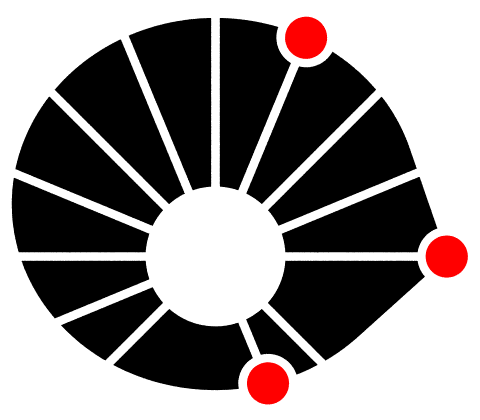
\includegraphics[width=0.2\textwidth]{unicamp_logo.png}\\[1cm] % Include a department/university logo - this will require the graphicx package
	
	\textsc{\LARGE Universidade Estadual de Campinas}\\[1.5cm] % Main heading such as the name of your university/college
	
	\textsc{\Large Instituto de Matemática, Estatística e Computação Científica}\\[0.5cm] % Major heading such as course name
	
	\textsc{\large MS211 - Calculo Numérico}\\[0.5cm] % Minor heading such as course title
	
	%------------------------------------------------
	%	Title
	%------------------------------------------------
	
	\HRule\\[0.4cm]
	
	{\huge\bfseries Relatório - Projeto SIR}\\[0.4cm] % Title of your document
	
	\HRule\\[1.5cm]
	
	%------------------------------------------------
	%	Author(s)
	%------------------------------------------------
	
	%\begin{minipage}{0.6\textwidth}
		\begin{flushleft}
			\large
			\textit{Alunos}\\
			Guido Neulaender - 217100 \\
			Heloisa Pimentel Lins de Silva - 236510 \\
			João Francisco Figueiredo Miranda - 218592 \\
			Rodrigo Ryan Oliveira da Silva - 244024 \\
			Silas Leonel Pereira Miranda - 258984
		\end{flushleft}
	%\end{minipage}
	~
	
	% If you don't want a supervisor, uncomment the two lines below and comment the code above
	%{\large\textit{Author}}\\
	%John \textsc{Smith} % Your name
	
	%------------------------------------------------
	%	Date
	%------------------------------------------------
	
	\vfill\vfill\vfill % Position the date 3/4 down the remaining page
	%\begin{minipage}{0.4\textwidth}
		\begin{flushright}
			\large
			\textit{Professor}\\
			Dr. Maicon Ribeiro Corrêa % Supervisor's name
		\end{flushright}
	%\end{minipage}
	
	{\large\today} % Date, change the \today to a set date if you want to be precise
	
	%------------------------------------------------
	%	Logo
	%------------------------------------------------
	 
	%----------------------------------------------------------------------------------------
	
	\vfill % Push the date up 1/4 of the remaining page
	
\end{titlepage}


\section{Introdução}
Esse projeto foi feito com intuito de compreender a evolução do coronavírus no Estado de Minas Gerais.
Nele foi utilizado o modelo compartimental SIR (Suscetíveis-Infectados-Removidos), que divide a população (N) em 3 grupos: suscetíveis a infecção (S); os que já foram infectados e que podem infectar os  (I); e os que já foram removidos (R), seja por terem sido curados ou pelo óbito. 
É sabido que esses 3 grupos interagem segundo o seguinte sistema de Equações Diferenciais Ordinárias (EDOs):
\[
	\od{S}{t} = - \gamma r_0 \frac{IS}{N} , \quad
	\od{I}{t} = \gamma \left( r_0 \frac{IS}{N} - I \right) \text{ e} \quad
	\od{R}{t} = \gamma I
\]
onde $r_0 = \frac{\beta}{\gamma}$ é constante ou dado em função do tempo. 
Para simulação desse sistema foi utilizado o método numérico de Runge-Kutta, que foi escolhido por ser um método bastante flexível, o que permite que sejam simulados  diversos cenários com diversas condições iniciais.
Vale ressaltar que foram utilizadas como base de dados as seguintes referências:
o painel coronavírus, organizado pelo Professor Alberto Saa \cite{git_saa};
o site da Wikipédia sobre \emph{Compartmental models in epidemiology} \cite{model}
e o livro Cálculo Numérico de Marcia A. G. Ruggiero e Vera L. R. Lopes \cite{calc_num}.
Ao final da pesquisa, conseguimos obter alguns resultados, disponibilizados em anexo ao final do relatório, que iremos discutir brevemente o que eles querem dizer e com toda implementação do código podendo ser encontrada no GitHub do grupo \cite{git_grupo}.

Para compreensão da evolução do coronavírus a partir do sistema de EDOs, dito anteriormente, foi-se avaliada duas possibilidades em relação ao $r_0$, a primeira com o seu valor constante e a segunda com seu valor variando em relação ao tempo.
Possivelmente, a principal diferença entre as duas possibilidades deve-se ao fato de que a segunda terá valores mais exatos do que a primeira, já que ela estará mudando sempre com o tempo devido a variação da taxa de infecção, enquanto a primeira terá sempre o mesmo valor independente das condições.

Para a primeira possibilidade, em que o $r_0$ é dito constante, adotamos seu valor como $r_0 \approx 2,6$, dado pela simples razão entre a taxa de infecção ($\beta \approx 0,34$) e a taxa de remoção ($\gamma \approx 0,13$).
Já a segunda possibilidade, que seria o $r_0$ em função do tempo, foi calculado a partir da seguinte fórmula, dados $\gamma$ e $\alpha$:
\[
	r_0(t) = \frac{1}{1 - \mu} + \frac{\ddot{C}}{\gamma \dot{C} (1 - \mu)}
	\text{, com} \quad
	\mu(t) = \frac{\alpha}{\gamma N} (\gamma C + \dot{C})
\]

\printbibliography

\end{document}

